\documentclass{article}
\usepackage[a4paper]{geometry}
\usepackage{tikz}
\usetikzlibrary{trees}

\title{Elements of Language Processing and Learning\\
Lab assignment \\
Stage 1: Computing the Probability of a Tree\\
Report}
\author{Benno Kruit, 10576223\\Sara Veldhoen, 10545298}

\begin{document}
\maketitle

The objective is to compute the probability of a parse tree, e.g. a tree in the test set. 


In general, the probability of a tree is the multiplication of the probability of the production, with the probabilities of the children. We actually compute the log probability to avoid arithmetic underflow due to the multiplication of small probabilities. Therefore, in the algorithm we perform an addition.
\begin{figure}
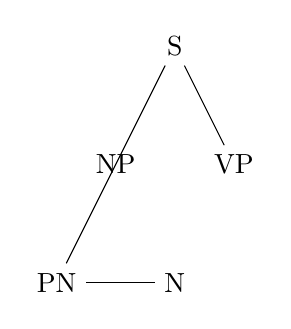
\begin{tikzpicture}

\node {S}
	child { node (left node) {NP}
		child {node (left node) {PN}}
		child {node (right node) {N}}
		}
	child {node (right node) {VP}}
    ;

\end{tikzpicture}
\caption{The probability of a tree is a multiplication of the probability of the production with the probability of its children}
\end{figure}

First step: annotate, call logScoreHelper
The function logScoreHelper essentially has two cases:\begin{itemize}
\item Basis: preterminal node. If the tree is a preterminal with one child, a leaf with a terminal (a word), the lexicon is called to compute the probability of this production. The probability of the children is not 
\item Recursive: internal node. If the tree is an inner node with trees as children, the grammar is called to compute the probability of the production. The probability of the children is computed via a recursive call to logScoreHelper.
A distinction is made between internal nodes with one or two children, thus calling the grammar for unary or binary rules respectively.
\end{itemize}
\end{document}